%% =========================================================================
%% Course Report Template (XeLaTex)
%% 
%% Author: 赵苡积 (Yunnan University, School of Information)
%% GitHub: https://github.com/yijizhao
%% 
%% =========================================================================
\documentclass{style/course-report}

\usepackage{subfigure}
\hypersetup{
    colorlinks=true,
    linkcolor=blue,
    filecolor=black,
    urlcolor=black,
    citecolor=blue,
}


% ================= 填写封面信息 =================
\coursetitle{《创新实验》开题报告} %课程报告标题
\expname{xxxxx} %题目
\studentname{成员1，成员2} %姓名
\studentid{20260001，20260002} %学号
\major{计算机科学与技术} %专业
\expdate{\today} %日期，默认当天，也可以根据自己需求修改

\begin{document}

% 生成封面
\makecover


\section{选题背景与意义}

描述选题的背景、动机与意义。适当引用政策文件\cite{YunNan}及国内外文献\cite{Chen2025IoVCrowdsensing,JTBH202106001}，阐明研究现状/动机，文献应尽量以近3年的为主。




\section{项目内容及目标}

本部分重点介绍计划做的内容，以及要达成的目标。建议采用总分形式，先概述总体内容和总目标，再列点分述子内容和子目标。


\section{方案设计}
% 本部分重点介绍针对要做的内容拟采取的技术方案

\subsection{方案概述}
搭配模型图/总体框架图/流程图等，描述设计思路、流程等。


\subsection{xxx模块}
分模块介绍：模块功能、形式化、示意图等。


\subsection{xxx模块}
分模块介绍：模块功能、形式化、示意图等。



\section{可行性分析}

从技术选型、已有基础（如数据（含出处/引用）、大创项目等）等角度分析可行性。

\section{创新点}

总结创新点

\section{成员分工及进度安排}

介绍成员分工及进展计划



公式示例，段内公式$a+b=c$，行间公式：
\begin{equation}
    \mathrm{ACC} = \frac{A}{B}
    \label{eq:acc}
\end{equation}

表格示例：
\begin{table}[H]
    \centering
    \caption{实验结果数据表} % 每个表格应有编号和标题，编号和标题应写在表格上方正中
    \begin{tabular}{ccc}
        \toprule
        参数 & 准确率 / \% & 训练时间 / s \\ % 表格中量与单位之间用“/”分隔
        \midrule
        设置 A & 92.5 & 120 \\
        设置 B & 95.1 & 180 \\
        \bottomrule
    \end{tabular}
    \label{tab:example}
\end{table} % 表格应为三线表

推荐使用python中的matplotlib绘图，加入自动裁剪命令，存为pdf，dpi设为300，注意图中文字应尽量使用中文。单图示例样式如下：
\begin{figure}[H]
    \centering
    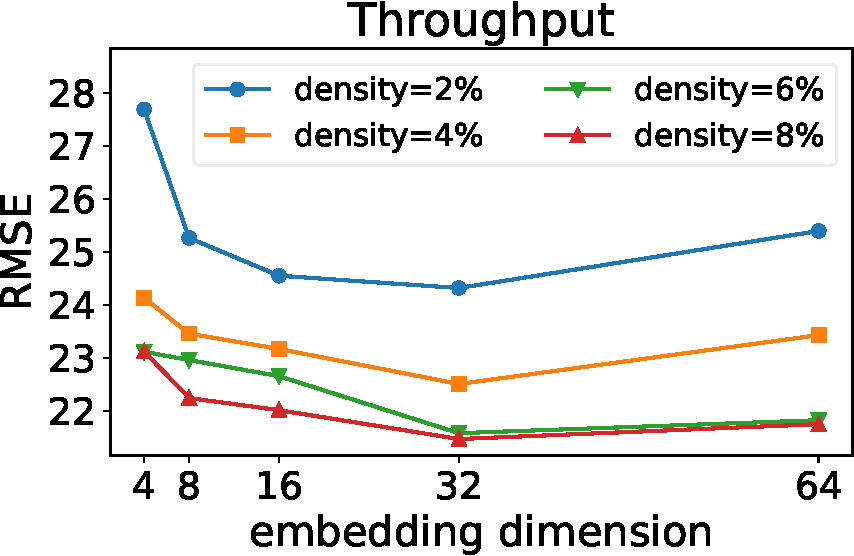
\includegraphics[width=0.70\textwidth]{figs/example.pdf}
    \caption{单图示例}
    \label{fig:example}
\end{figure}

多图并列示例图表样式如下：
%%%%%%%%%%%%%%%%%%%%%%%%%%%%%%%%%%%%%%%%%%%%
%                 Figure                  %
%%%%%%%%%%%%%%%%%%%%%%%%%%%%%%%%%%%%%%%%%%%%
\begin{figure}[ht]
    \centering
    \subfigure[XXX1曲线]{
        \label{fig:example_a}
        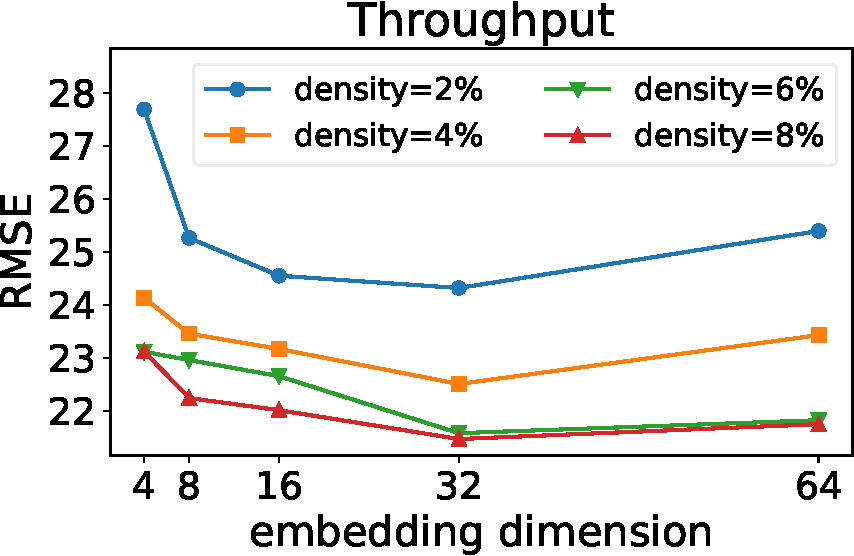
\includegraphics[width=0.45\linewidth]{figs/example.pdf}
    }\hfill
    \subfigure[XXX2曲线]{
        \label{fig:example_b}
        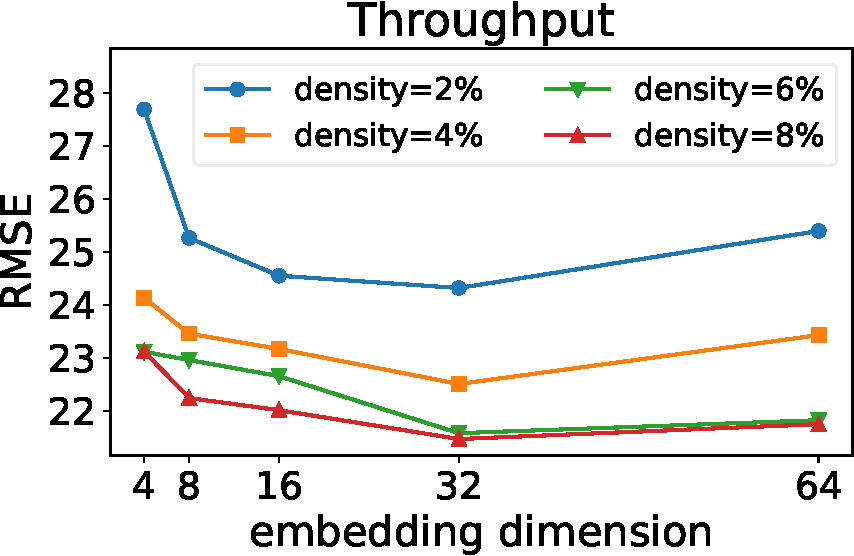
\includegraphics[width=0.45\linewidth]{figs/example.pdf}
    }\hfill
    \subfigure[XXX3曲线]{
        \label{fig:example_c}
        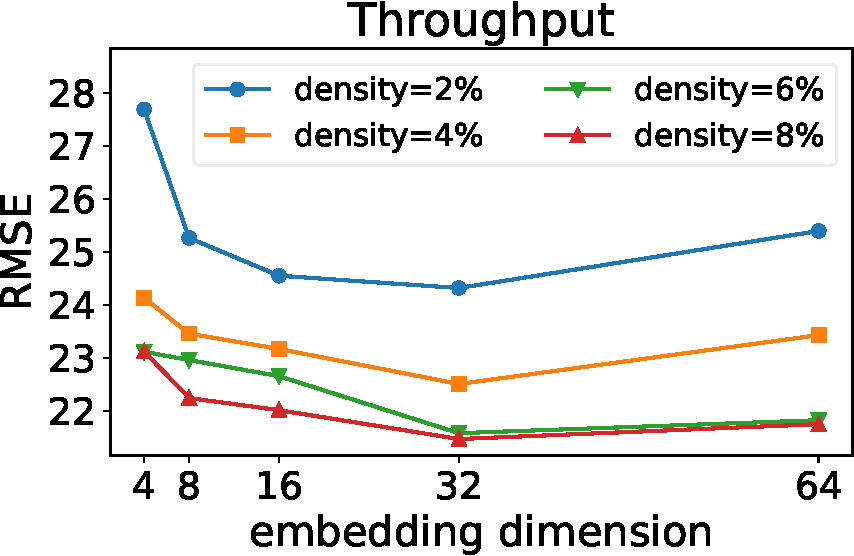
\includegraphics[width=0.45\linewidth]{figs/example.pdf}
    }\hfill
    \subfigure[XXX4曲线]{
        \label{fig:example_d}
        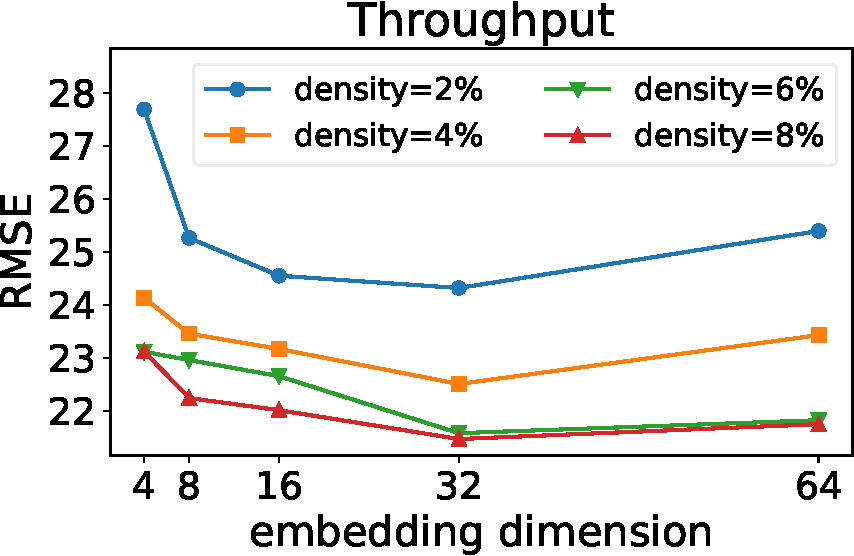
\includegraphics[width=0.45\linewidth]{figs/example.pdf}
    }
    \caption {\label{fig:multi1}多图示例.}
\end{figure}

图、表、公式、算式等，一律用阿拉伯数字分别依序连续编排序号，其标注形式应便于互相区别，可分别为：图\ref{fig:example}、图\ref{fig:example_a}、表\ref{tab:example}、公式\ref{eq:acc}等。


 
\bibliography{ref}
% 参考文献主要包含实验过程中涉及到的参考资料或者借鉴别人的材料等，如无可删除本节。 



\end{document}